\section{October 12, 2015}

\subsection{Cauchy's Theorem}

\begin{thm}[Cauchy]
Suppose $G$ is a finite group and there is a prime $p \mid \lvert Z(G)
\vert$. Then $G$ has an element of order $p$.
\end{thm}

\begin{proof}
We wish to show that $\exists a \st a^p = e$. Consider the subset of
$G^p$ such that all elements multiply to $e$, or
\[ X = \lbrace (a_1, \dots, a_p) \mid a_i \in G, a_1 a_2 \cdots a_n = e
\rbrace. \]
We wish to show that $\exists a \in G \st (a, \dots, a) \in X$. First we
trivially establish the fact that $X$ is nonempty.

Consider the function $f : G^p \to G^p$ given by $(g_1, \dots, g_p)
\xmapsto{f} (g_p, g_1, \dots, g_{p - 1})$. This is clearly a bijection
within $X$. In fact, we hav $f^p = \id_X, f \in \aut(X)$ and we can
define the map $\ZZ / p \ZZ \to \aut(X), [k] \mapsto f^k$ as an
injective homomorphism, which in turn gives us an action on $X$. Namely
$[k] \cdot x = f^k(x)$. This turns to problem into showing that $\exists
x \in X \st [k]x = x \quad \forall [k] \in \ZZ / p \ZZ$.

Notice that the map $G^{p - 1} \to X, (g_1, \dots, g_{p - 1}) \mapsto
(g_1, \dots, g_{p - 1}, (g_1 \cdots g_{p - 1})^{-1})$ is a bijection, so
we have $\lvert X \rvert = \lvert G^{p - 1} \rvert$. Because $p \mid
\lvert G \rvert$, we have $p \mid \lvert X \rvert$ as well.

Also notice that
\[ \forall x \in X \quad \lvert \ZZ / p \ZZ \cdot x \rvert \mid \lvert
\ZZ / p \ZZ \rvert = p \]
by \ref{orbitstabilizer} (Orbit Stabilizer Theorem), which implies that
$\lvert \ZZ / p \ZZ \cdot x \rvert = 1, p$.

Let $n$ be the number of singleton orbits and let $l$ be the number of
orbits with $p$ elements. Then we have $p \mid \lvert X \rvert = n + lp
\implies p \mid n$. We also have $n \geq 1$ because $(e, e, \dots, e)
\in X$ is fixed. $n > 1$ because $p \mid n$. This means that $f$ fixes
$(g_1, g_2, \dots, g_p) \xmapsto{f} (g_p, g_1, \dots, g_{p - 1}),
\prod_i g_i = e \implies g_1 = g_2 = \cdots = g_p \neq e$.
\end{proof}

\subsection{Semidirect Products}
\begin{df}
\label{sdprod}
Given a group $G, H \leq G, N \lhd G$, the following statements are
equivalent.
\begin{itemize}
\item $G = NH$ and $N \cap H = \lbrace e \rbrace$.
\item Every element in $G$ can be written as a product $nh$ with $n \in
N, h \in H$.
\item Every element in $G$ can be written as a product $hn$ with $n \in
N, h \in H$.
\item The natural embedding $H \to G$ composed with the natural
projection $G \to G / N$ yields an isomorphism between $H$ and $G / N$.
\item There is a homomorphism $G \to H$ that is the identity on $H$ and
whose kernel is $N$.
\end{itemize}
If one, and therefore all these statements hold, then we say that $G$ is
the \textbf{semidirect product} of $N$ and $H$, written
\[ G = N \rtimes H. \]
This is also said $G$ \textbf{splits} over $N$.
\end{df}

\begin{ex}
Recall that $D_{2n} = \lbrace \rho, \tau \mid \rho^n = e = \tau^2, \tau
\rho = \rho^{-1} \tau \rbrace$ and that $\cycgroup{\rho}$ is normal in
$D_{2n}$ but $\cycgroup{\tau}$ is not. We also have the following
conditions:
\begin{enumerate}
\item $\cycgroup{\rho} \cap \cycgroup{\tau} = \lbrace e \rbrace$.
\item $\forall g \in D_{2n} \quad \exists! \rho^k \in \cycgroup{\rho},
\tau^l \in \cycgroup{\tau} \st g = \rho^k \tau^l$.
\end{enumerate}
so we can write $D_{2n} = \cycgroup{\rho} \rtimes \cycgroup{\tau}$.
\end{ex}

\begin{note}
We present a change of notation. $\aut_{\textrm{set}}(G)$ will be the
automorphism group of the underlying set of $G$, and we will require
that $\aut(G)$ consist only of isomorphisms. In these notes, I will be
completely unambiguous and $\aut(X)$ will refer to structure preserving
morphisms from $X \to X$ and $\sym(X)$ will refer to the automorphism
group of the underlying set.

To be precise, $f \in \sym(X)$ requires the following diagrams to
commute.
\[ 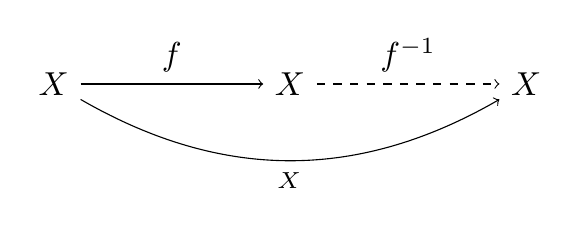
\begin{tikzpicture}[scale=3, nodes={scale=1.2}]
\node (X1)  at (0, 0) {$X$};
\node (X2)  at (1, 0) {$X$};
\node (X3)  at (2, 0) {$X$};

\path[->] (X1) edge             node[above]{$f$}        (X2)
          (X2) edge[dashed]     node[above]{$f^{-1}$}   (X3)
          (X1) edge[bend right] node[below]{$\id_X$}    (X3);
\end{tikzpicture} \qquad 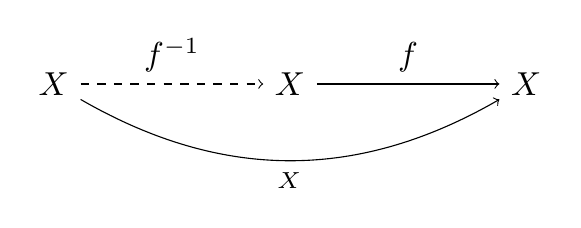
\begin{tikzpicture}[scale=3, nodes={scale=1.2}]
\node (X1)  at (0, 0) {$X$};
\node (X2)  at (1, 0) {$X$};
\node (X3)  at (2, 0) {$X$};

\path[->] (X2) edge             node[above]{$f$}        (X3)
          (X1) edge[dashed]     node[above]{$f^{-1}$}   (X2)
          (X1) edge[bend right] node[below]{$\id_X$}    (X3);
\end{tikzpicture} \]

Additionally, $f \in \aut(X)$ requires that $f \in \sym(X)$ and $f$
preserves whatever structure $X$ has. Suppose $X$ is a group/ring/field.
Then for each operation $*$, we require the following diagram to commute
as well.
\[ 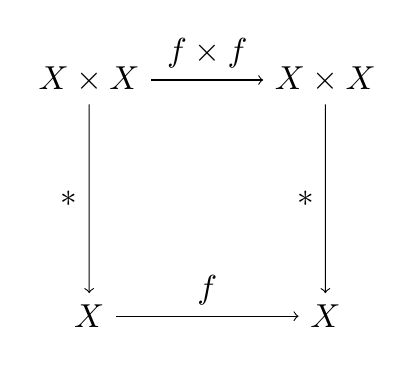
\begin{tikzpicture}[scale=3, nodes={scale=1.2}]
\node (XX1) at (0, 1) {$X \times X$};
\node (XX2) at (1, 1) {$X \times X$};
\node (X1)  at (0, 0) {$X$};
\node (X2)  at (1, 0) {$X$};

\path[->]
(XX1) edge node[above]{$f \times f$}    (XX2)
(XX1) edge node[left] {$*$}             (X1)
(X1)  edge node[above]{$f$}             (X2)
(XX2) edge node[left] {$*$}             (X2);
\end{tikzpicture} \]
\end{note}

Anyways, we now explore what exactly we mean in
definition~\ref{sdprod}. Suppose $N, A$ are two subgroups so that $f : N
\times A \to G, (n, a) \xmapsto{f} na$ is a bijection. This implies that
every element in $g \in G$ can be written uniquely as $g = na, n \in N,
a \in A$.  It also implies that $N \cap A = \lbrace e \rbrace$, because
$g \in N \cap A \implies g = e_N g_A = g_N e_G$ and uniqueness gives $g
= e$. Now suppose further that $N \lhd G$. Then we have $\forall n_1,
n_2 \in N, a_1, a_2 \in A$,
\[ \begin{aligned}
(n_1 a_1)(n_2 a_2) &= n_1 a_1 n_2 a_1^{-1} a_1 a_2 \\
\implies f^{-1}(f(n_1, a_1) \cdot f(n_2, a_2)) &= (n_1 (a_1 n_2
a_1^{-1}), a_1 a_2) \\
\implies f(n_1, a_1) \cdot f(n_2, a_2) &= f(n_1 (a_1 n_2 a_1^{-1}), a_1
a_2), \\
\end{aligned} \]
so $f$ is a isomorphism only if we define the multiplication on $N
\times A$ to be $(n_1, a_1)(n_2, a_2) = (n_1 (a_1 n_2 a_1^{-1}), a_1
a_2)$.

$N$ is also normal in $G$ so we can say that $A$ acts on $N$ by
conjugation.
